\documentclass[11pt, reqno]{amsart}

\input{~/latex-common/macros.tex}
\usepackage[backend=bibtex,style=science]{biblatex}
% \bibliography{main.bib}
\pgfplotsset{compat=1.18}

\pagestyle{fancy}                         % fancy (allow headers, footers)
\fancyhf{}                                % clear all header/footer settings.
\cfoot{\thepage}                          % set page-numbers in footer.
% \lhead{\textit{\textbf{ Amittai, S}}}   % set name in header, left.
% \rhead{\textsc{Math 71: Algebra}}       % set class name in header, right.
\renewcommand{\headrulewidth}{0pt}
\renewcommand{\footrulewidth}{0pt}


\renewcommand{\theenumi}{\alph{enumi}}

\begin{document}

\newdate{due-date}{23}{05}{2023}

\title{CS-89.31: Deep Learning Generalization and Robustness\\ Amittai Siavava \\ \displaydate{due-date}}
\author{Amittai Siavava}
% \date{\today}


\setlength{\headheight}{13.0pt}
\setlength{\footskip}{15.0pt}

\maketitle

\bigskip

\def \cram { \textsc{cram} }
\def \dom { \textsc{domineering} }
\def \sub { \textsc{subtraction} }
\def \weighted { \textsc{weighted odds and evens}}
\def \nim { \textsc{nim} }
\def \P { \mathbf{P}}
\def \N { \mathbf{N}}

\section{Adversarial Training}

Adversarial training took about $2$ hours on my laptop (which has a quite capable GPU).
The general trend was improvement in both the benign and adversarial test accuracies
the more the model was trained. However, the rate of improvement slowed down and became almost
zero, suggesting that the methods used would reach a limit and perhaps
other methods would be needed to improve the model further.

\step
\begin{figure}[h!]
  \centering
  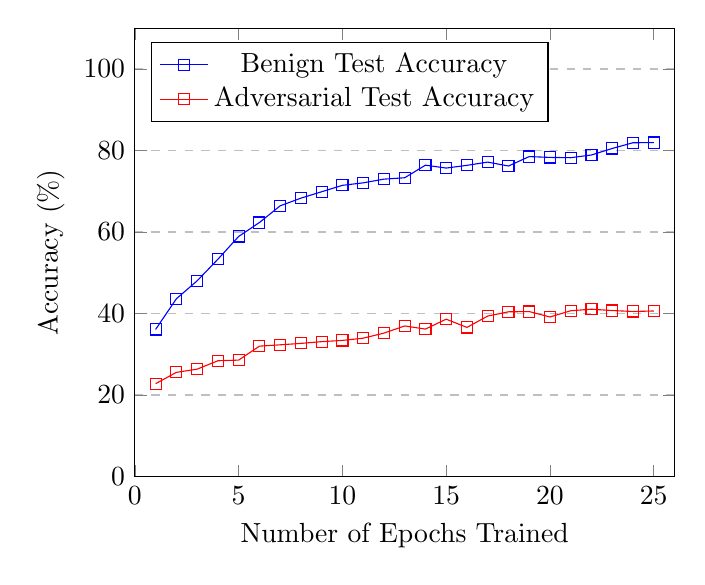
\begin{tikzpicture}
    \begin{axis}[
      xlabel={Number of Epochs Trained},
      ylabel={Accuracy $(\%)$},
      xmin=0, xmax=26,
      ymin=0, ymax=110,
      xtick={0,5,10,15,20,25},
      ytick={0,20,40,60,80,100},
      legend pos=north west,
      ymajorgrids=true,
      grid style=dashed,
      ]
      \addplot[
      color=blue,
      mark=square,
      ]
      coordinates {
        (1,36.10)(2,43.62)(3,48.02)(4,53.31)(5,58.91)(6,62.32)(7,66.42)(8,68.31)(9,69.88)(10,71.45)(11,72.06)(12,72.97)(13,73.31)(14,76.40)(15,75.69)(16,76.36)(17,77.15)(18,76.19)(19,78.51)(20,78.30)(21,78.23)(22,78.90)(23,80.50)(24,81.90)(25,81.94)
      };
      \addlegendentry{Benign Test Accuracy}
      \addplot[
      color=red,
      mark=square,
      ]
      coordinates {
        (1,22.78)(2,25.56)(3,26.35)(4,28.41)(5,28.57)(6,31.99)(7,32.32)(8,32.67)(9,33.10)(10,33.40)(11,33.95)(12,35.19)(13,36.95)(14,36.18)(15,38.61)(16,36.59)(17,39.38)(18,40.42)(19,40.48)(20,39.15)(21,40.68)(22,41.06)(23,40.73)(24,40.50)(25,40.62)
      };
      \addlegendentry{Adversarial Test Accuracy}
    \end{axis}
  \end{tikzpicture}
  \caption{Adversarial Training: Model Performance vs. Epochs Trained}~\label{fig:results}
\end{figure}

\newpage


\begin{table}[h!]
    \centering
    \begin{tabular}{| r | r | r |}
      \bottomrule
      \textbf{Number of Epochs}   & \textbf{Benign Test Accuracy}  & \textbf{Adversarial Test Accuracy} \\   
      \midrule
      $1$                         & $36.10$                 & $22.78$ \\
      $2$                         & $43.62$                 & $25.56$ \\
      $3$                         & $48.02$                 & $26.35$ \\
      $4$                         & $53.31$                 & $28.41$ \\
      $5$                         & $58.91$                 & $28.57$ \\
      $6$                         & $62.32$                 & $31.99$ \\
      $7$                         & $66.42$                 & $32.32$ \\
      $8$                         & $68.31$                 & $32.67$ \\
      $9$                         & $69.88$                 & $33.10$ \\
      $10$                        & $71.45$                 & $33.40$ \\
      $11$                        & $72.06$                 & $33.95$ \\
      $12$                        & $72.97$                 & $35.19$ \\
      $13$                        & $73.31$                 & $36.95$ \\
      $14$                        & $76.40$                 & $36.18$ \\
      $15$                        & $75.69$                 & $38.61$ \\
      $16$                        & $76.36$                 & $36.59$ \\
      $17$                        & $77.15$                 & $39.38$ \\
      $18$                        & $76.19$                 & $40.42$ \\
      $19$                        & $78.51$                 & $40.48$ \\
      $20$                        & $78.30$                 & $39.15$ \\
      $21$                        & $78.23$                 & $40.68$ \\
      $22$                        & $78.90$                 & $41.06$ \\
      $23$                        & $80.50$                 & $40.73$ \\
      $24$                        & $81.90$                 & $40.50$ \\
      $25$                        & $81.94$                 & $40.62$ \\
    \toprule
  \end{tabular}
  \caption{Adversarial Training: Model Performance vs. Epochs Trained}~\label{tab:results}
\end{table}


\pagebreak
\section{Data Augmentation}

In the data augmentation part, my results seemed to deteriorate initially when I introduce new
augmentation techniques, but the results would sometimes do better than earlier models
after significant training.
I think this is because when new augmentation techniques are introduced, the model
initially encounters a lot of images that it does not ``know'' how to properly classify yet,
so it assigns them labels in an almost random manner. This reduces the accuracy.
However, with more training, the model learns how to properly classify these new images
and actually becomes better at classifying the original dataset,
hence the test accuracy is overall better.

However, with too many augmentation techniques, the model performance starts decreasing again.
I think this is because the augmentation introduces too much noise in the dataset
than the network can handle and either:
\begin{enumarabic}
  \item The model overfits the training data, but performs worse on the test data.
  \item The model does not learn how to classify the images properly in the number of epochs trained.
\end{enumarabic}

\step
\begin{table}[h!]
  \centering
  \begin{tabular}{|l|r|r|r|}
    \bottomrule
    Mode & 10 Epochs & 30 Epochs & 50 Epochs \\
    \midrule
    Tech0 & $0.31409090161323455$ & $0.55854935935839753$ & $0.6845454575483436$ \\
    Tech1 & $0.24508402584390405$ & $0.45590909123420715$ & $0.7595454421496957$ \\
    Tech2 & $0.16699999910593033$ & $0.23999999701976776$ & $0.5295454454421997$ \\
    Tech3 & $0.09045454859733582$ & $0.13590909540653623$ & $0.3357935293577323$ \\
    \toprule
  \end{tabular}
  \caption{Training Results with Data Augmentation}~\label{tab:augmentation-results}
\end{table}

% Plot
\begin{figure}[h!]
  \centering
  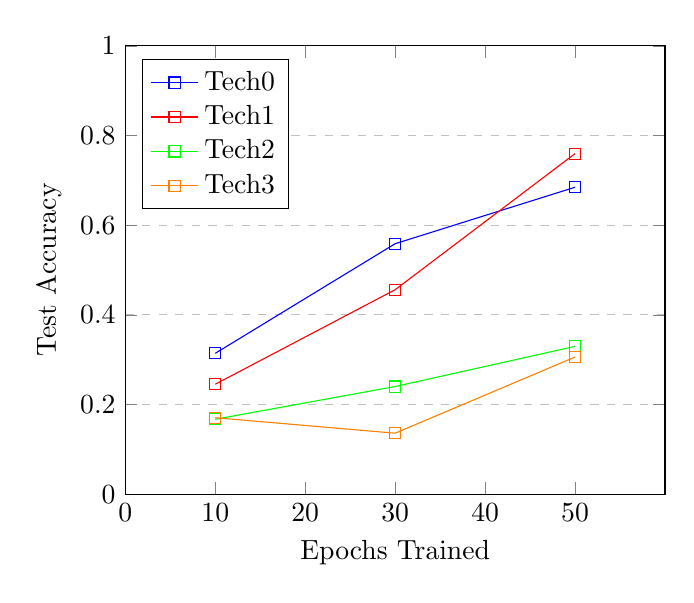
\begin{tikzpicture}
    \begin{axis}[
      xlabel={Epochs Trained},
      ylabel={Test Accuracy},
      xmin=0, xmax=60,
      ymin=0, ymax=1,
      xtick={0,10,20,30,40,50},
      ytick={0,0.2,0.4,0.6,0.8,1.0},
      legend pos=north west,
      ymajorgrids=true,
      grid style=dashed,
      ]
      \addplot[
      color=blue,
      mark=square,
      ]
      coordinates {
        (10,0.31409090161323455)(30,0.55854935935839753)(50,0.6845454575483436)
      };
      \addlegendentry{Tech0}
      \addplot[
      color=red,
      mark=square,
      ]
      coordinates {
        (10,0.24508402584390405)(30,0.45590909123420715)(50,0.7595454421496957)
      };
      \addlegendentry{Tech1}
      \addplot[
      color=green,
      mark=square,
      ]
      coordinates {
        (10,0.16699999910593033)(30,0.23999999701976776)(50,0.3295454454421997)
      };
      \addlegendentry{Tech2}
      \addplot[
      color=orange,
      mark=square,
      ]
      coordinates {
        (10,0.17045454859733582)(30,0.13590909540653623)(50,0.3057935293577323)
      };
      \addlegendentry{Tech3}
    \end{axis}
  \end{tikzpicture}
  \caption{Data Augmentation: Model Performance vs. Epochs Trained}~\label{fig:augmentation-results}
\end{figure}


% \end{problem}
\end{document}
